\documentclass[11pt, oneside]{article}   	% use "amsart" instead of "article" for AMSLaTeX format
\usepackage[margin=1in]{geometry}                		% See geometry.pdf to learn the layout options. There are lots.
\geometry{letterpaper}                   		% ... or a4paper or a5paper or ... 
%\geometry{landscape}                		% Activate for rotated page geometry
%\usepackage[parfill]{parskip}    		% Activate to begin paragraphs with an empty line rather than an indent
\usepackage{graphicx}				% Use pdf, png, jpg, or eps§ with pdflatex; use eps in DVI mode
								% TeX will automatically convert eps --> pdf in pdflatex		
\usepackage{amssymb}
\usepackage{courier}
%usepackage{undertilde}
\usepackage[numbered,framed]{matlab-prettifier}
\usepackage{framed}

\usepackage[T1]{fontenc}
\usepackage{mathtools}  % loads »amsmath«
\usepackage{physics}
\usepackage{listings}

\lstset{
  language=C,                % choose the language of the code
  numbers=left,                   % where to put the line-numbers
  stepnumber=1,                   % the step between two line-numbers.        
  numbersep=5pt,                  % how far the line-numbers are from the code
  backgroundcolor=\color{white},  % choose the background color. You must add \usepackage{color}
  showspaces=false,               % show spaces adding particular underscores
  showstringspaces=false,         % underline spaces within strings
  showtabs=false,                 % show tabs within strings adding particular underscores
  tabsize=2,                      % sets default tabsize to 2 spaces
  captionpos=b,                   % sets the caption-position to bottom
  breaklines=true,                % sets automatic line breaking
  breakatwhitespace=true,         % sets if automatic breaks should only happen at whitespace
  title=\lstname,                 % show the filename of files included with \lstinputlisting;
}

\setlength{\parskip}{0.5em}

%SetFonts
\newcommand\Rey{\mbox{\textit{Re}}}

\title{\vspace{-6ex}\large PHYS 516: Methods of Computational Physics \\ [1ex]
 ASSIGNMENT 6- TIGHT BINDING MODEL OF ELECTRONIC STRUCTURES\vspace{-3ex}}
\author{Anup V Kanale}
\date{\vspace{-3ex}\today}							% Activate to display a given date or no date

\begin{document}
\vspace{-6ex}\maketitle

\section{The Hamiltonian Matrix}
A programw as written to set up the Hamiltonian matrix and diagonalize it using the functions \texttt{tred2.c} and \texttt{tqli.c} from the book \textit{Numerical Recipes}. The code is attached in the appendix, along with the plotting codes.

\section{Effect of lattice constants on density of state}
 The density of states (DOS) of a system describes the number of states per interval of energy at each energy level that are available to be occupied. It is given by 
 	\begin{equation}
 	D(\varepsilon) = \sum \limits_{\nu=1}^{n4} \frac{1}{\sqrt{\pi}\sigma} \exp (\frac{-(\varepsilon - \varepsilon_\nu)^2}{\sigma^2})
 	\end{equation}
 where $\sigma = 0.1 eV$ is the energy spread given to each energy eigenvalue, $\varepsilon_\nu$. The following parameters were used: \texttt{InitUcell[0] = InitUcell[1] = InitUcell[2] = 1}, \texttt{nAtoms = 8} and \texttt{LCNS = 1.8 $\times$ 5.43 $A$, 1.4 $\times$ 5.43 $A$, 1 $\times$ 5.43 $A$}, \texttt{$k_BT$ = 0.2 eV}.
 
 The plots below show the Density of States for different lattice constant values. We see that when the lattice contant is the largest (\texttt{LCNS = 1.8 $\times$ 5.43 $A$}), there are two sharp peaks, which means that when the atoms are furthest from each other, the density is high in the energy states $E_s$ and $E-p$ and zero everywhere else.
 
 When LCNS reduces slightly, the atoms are closer together and the density in the states in between increases.
 
 For the case with the least LCNS ((\texttt{LCNS = 1.0 $\times$ 5.43 $A$})), the atoms are very close together so the energy states in between also start getting populated.

	\begin{figure}[!htbp]
	\centering
	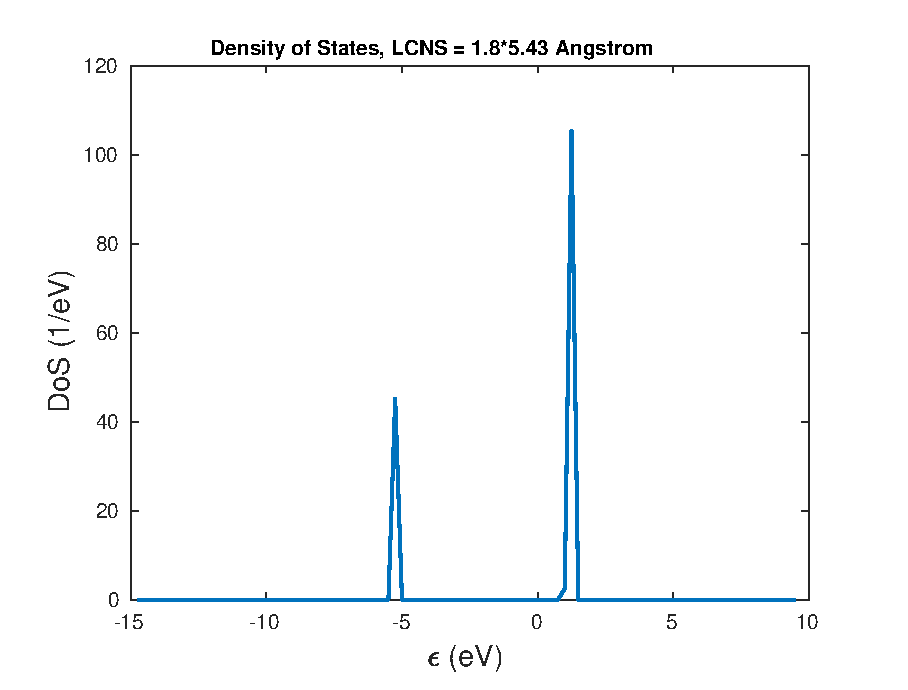
\includegraphics[scale=0.55]{dos_1pt8.eps}
	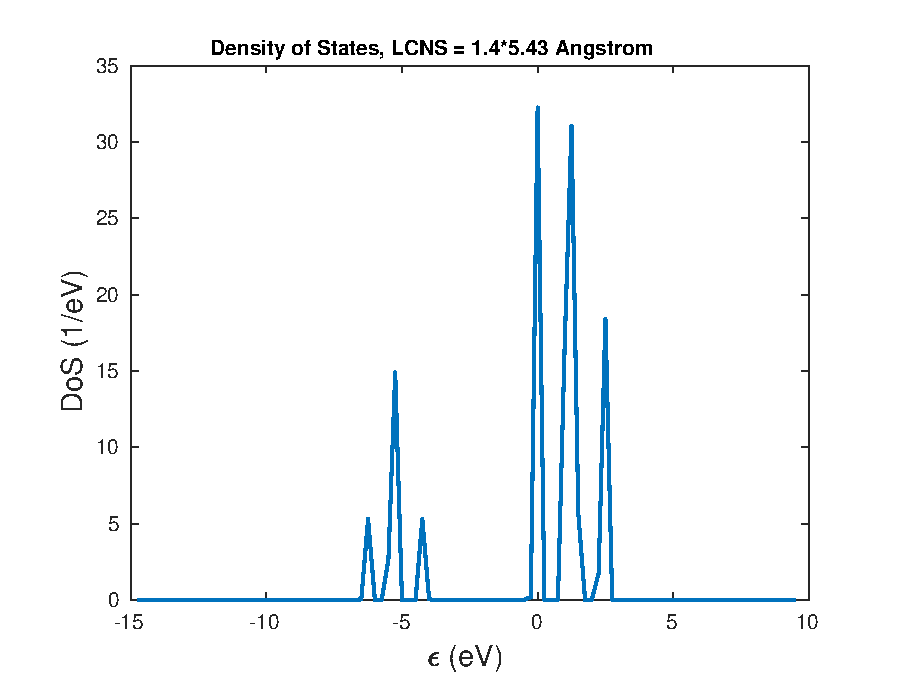
\includegraphics[scale=0.55]{dos_1pt4.eps}
	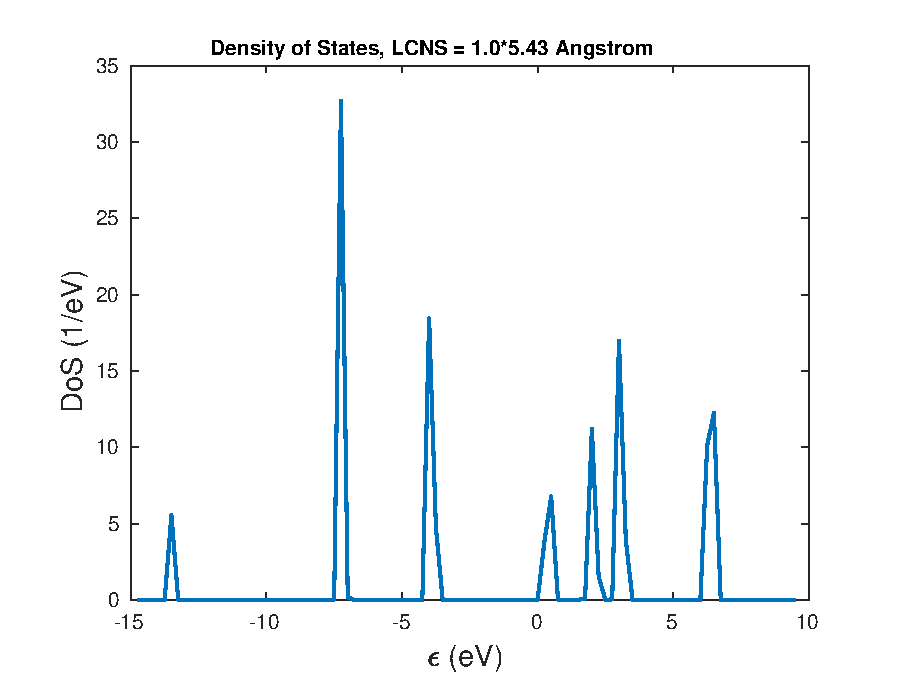
\includegraphics[scale=0.55]{dos_1pt0.eps}
	\caption{Density of States for 8 atoms}
	\end{figure}


\section{Effect of number of atoms on density of state}
The Density of states with a different number of periodic unit cells, i.e., a different number of atoms was plotted as shown in the figure below, for \texttt{LCNS = 1.0 $\times$ 5.43 $A$}. We see that the density of states has  a larger spread now as more atoms interact with each other.
	\begin{figure}[!htbp]
	\centering
	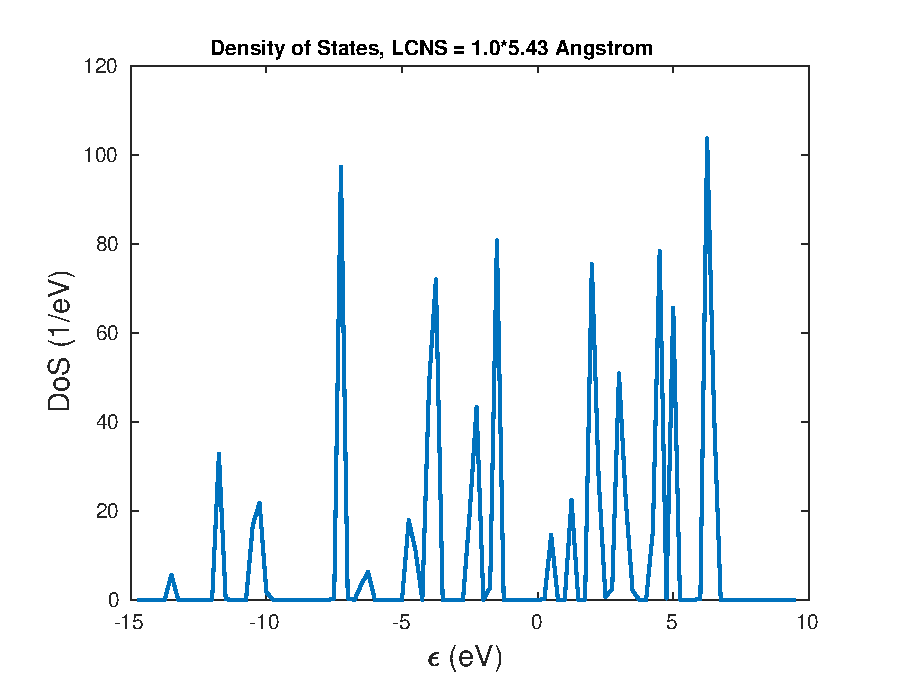
\includegraphics[scale=0.55]{dos_1pt0_Ucell2.eps}
	\caption{Density of States for 64 atoms}
	\end{figure}


\section{Fermi Distribution}
Fermi distribution represents the probablity of a state of energy being occupied by an electron. It is given by
	\begin{equation}
	f({\varepsilon_\nu}) = \frac{2}{ \exp{\frac{\varepsilon_\nu - \mu}{k_BT}} +1}
	\end{equation}

I calculate the Fermi energy by first finding the chemical potential $\mu$ using Newton-Raphson method, using the fact that the integral of the distribution over energy gives the total number of electrons. Mathetically,
	\begin{equation}
	\sum \limits_\nu f({\varepsilon_\nu}) = 4N
	\end{equation}
The parameters used for the simulation were: \texttt{InitUcell[0] = InitUcell[1] = InitUcell[2] = 2}, \texttt{nAtoms = 64}, \texttt{LCNS = 5.43 $A$}, \texttt{$k_BT$ = 0.2 eV} and \texttt{eigenenergies = 256}.
The plot below shows the distribution
	\begin{figure}[!htbp]
	\centering
	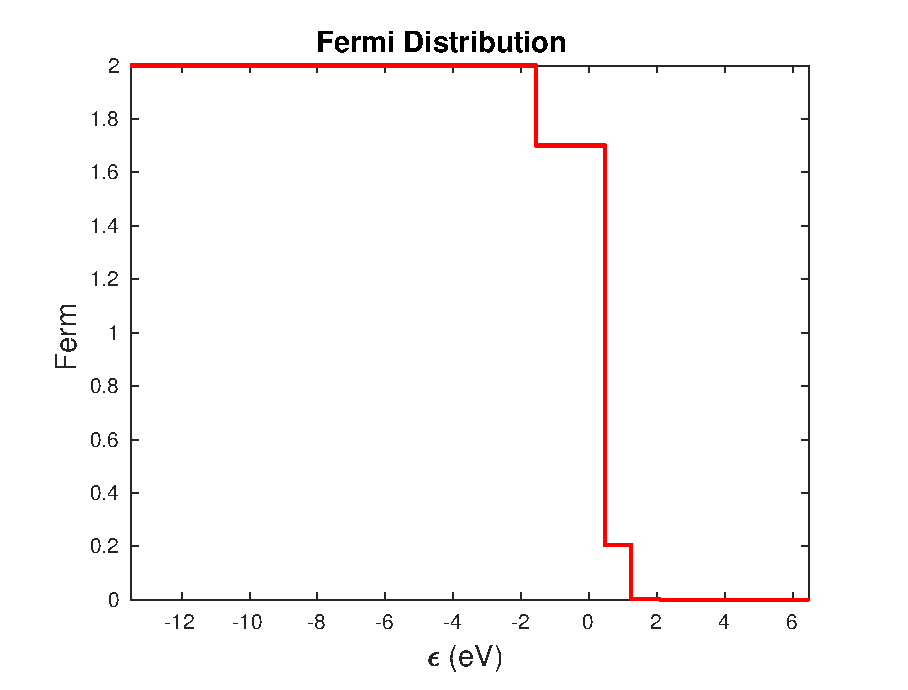
\includegraphics[scale=0.5]{fermiDist.eps}
	\end{figure}

\pagebreak
\appendix
\section{C Program}
\lstinputlisting[language=C, frame=single]{siCrystal.c}
\lstinputlisting[style=Matlab-editor]{siCrystal_Plot.m}

\end{document}